\usetikzlibrary{arrows}
\tikzstyle{myedgestyle} = [-open triangle 45]

\begin{tikzpicture}

\node at (-0.225,0.075) {Domain};
\draw  (-0.975,0.525) rectangle (0.5,-0.375);
\node at (-0.25,-2.55) {Formal};
\node at (-0.25,-2.925) {Model};
\draw  (-0.975,-2.325) rectangle (0.525,-3.15);
\draw (-0.825,-2.325) edge[-latex,dashed] (-0.825,-0.375);
\node at (3,0.075) {Metamodel};
\draw  (2.025,0.525) rectangle (3.975,-0.375);
\draw (2,0.375) edge[-latex, dashed] (0.5,0.375);
\draw (1.5,-0.25) edge[-{open diamond}] (0.5,-0.25) -- (1.5,-1) -- (0.25,-1) edge[-latex] (0.25,-0.375);
\node at (0.5,-0.5) {\tiny{0..*}};
\node at (0.875,-0.875) {\tiny{Subdomain}};
\draw (-0.225,-2.325) edge[dashed] (-0.225,-1.65);
\draw (-0.225,-1.65) edge[dashed] (2.25,-1.65);

\draw (2.25,-1.65) edge[dashed, -latex] (2.25,-0.375);
\node at (0.9,-1.5) {\tiny{<<instanceof>>}};
\node at (1.25,0.5) {\tiny{concepts of}};
\node at (1.25,0.625) {\tiny{relevant}};
\node at (1.25,0.75) {\tiny{describes}};

\draw  (5.175,0.525) rectangle (6.825,-0.375);
\node at (6,0.075) {
\includegraphics[width=0.01\textwidth]{../graphics/concept.png} {\fontsize{8}{6}\selectfont Structure}};
\draw (3.975,0.075) edge[open diamond-latex] (5.175,0.075);

\node at (6,-1.2) {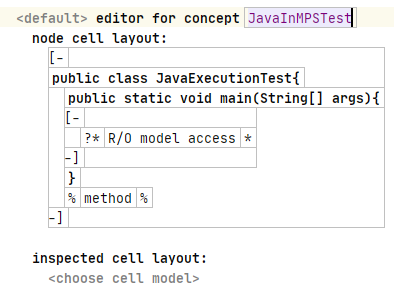
\includegraphics[width=0.01\textwidth]{../graphics/editor.png} {\fontsize{6}{6}\selectfont Editor}};
\node at (6,-1.425) {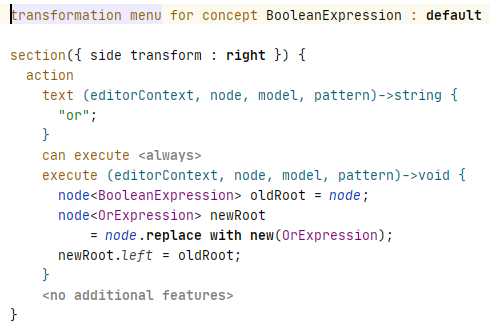
\includegraphics[width=0.01\textwidth]{../graphics/transformation.png} {\fontsize{6}{6}\selectfont Transform.}};
\node at (6,-1.65) {
\includegraphics[width=0.007\textwidth]{../graphics/intentions.png} {\fontsize{6}{6}\selectfont Intentions}};
\draw  (5.175,-1.05) rectangle (6.825,-1.8);
\draw (6,-1.05) edge[dashed, -open triangle 45] (6,-0.375);

\draw (0.3,-2.325) edge[dashed] (0.3,-2.025);
\draw (0.3,-2.025) edge[dashed] (3.75,-2.025);
\draw (3.75,-2.025) edge[dashed] (3.75,-1.425);
\draw (3.75,-1.425) edge[dashed, -latex] (5.175,-1.425);
\node at (2.1,-2.175) {\tiny{expressed by means of}};

\node at (6,-2.7) {Semantics};
\draw  (5.175,-2.325) rectangle (6.825,-3.15);
\draw (0.525,-2.775) edge[dashed, -latex] (5.175,-2.775);

\node at (9.075,0.225) {Static};
\node at (9.075,-0.075) {Semantics};
\draw  (8.175,0.525) rectangle (9.9,-0.375);
\draw (8.175,0.075) edge[dashed, -latex] (6.825,0.075);
\node at (7.5,0.225) {\tiny{means of}};
\node at (7.5,0.375) {\tiny{expressed by}};

\draw (3,0.525) edge[open diamond-] (3,0.9);
\draw (3,0.9) edge (9.075,0.9);
\draw (9.075,0.9) edge[-latex] (9.075,0.525);

\node at (9.075,-1.425) {DSL};
\draw  (8.175,-1.05) rectangle (9.9,-1.8);
\draw (9.075,-1.05) edge[open diamond-] (9.075,-0.675);
\draw (9.075,-0.675) -- (3.6,-0.675);
\draw (3.6,-0.675) edge[-latex] (3.6,-0.375);

\draw (8.175,-1.425) edge[open diamond-latex] (6.825,-1.425);
\draw (8.175,-1.8) edge[open diamond-latex] (6.825,-2.325);

\node at (9.075,-2.55) {Modelling};
\node at (9.075,-2.925) {Language};
\draw  (8.175,-2.325) rectangle (9.9,-3.15);
\node at (9,-2.1) {\tiny{<<synonym>>}};
\draw (9,-2.325) -- (9,-2.175);
\draw (9,-1.8) -- (9,-2.025);

\draw (-0.225,-3.15) edge[dashed] (-0.225,-3.525) ;
\draw  (-0.225,-3.525) edge[dashed] (10.5,-3.525);
\draw (10.5,-3.525) edge[dashed] (10.5,0.075);
\draw (10.5,0.075) edge[dashed, -latex] (9.9,0.075);
\node at (2.25,-3.375) {\tiny{respects}};
\end{tikzpicture}